\documentclass[14pt]{article}
\usepackage[utf8]{inputenc}
\usepackage[T2A]{fontenc}
\usepackage[russian]{babel}
\usepackage{amsmath, amssymb}
\usepackage{geometry}
\usepackage{graphicx}
\usepackage{xcolor}
\usepackage{hyperref}
\usepackage{tasks}
\usepackage{tcolorbox}
\tcbuselibrary{skins, breakable}
\usepackage{fancyhdr}
\usepackage{lastpage}
\usepackage{enumite

% O‘zbek tilidagi tangens va kotangens uchun maxsus buyruqlar
\newcommand{\tg}{\operatorname{tg}}
\newcommand{\ctg}{\operatorname{ctg}}

% Geometriya sozlamalari
\geometry{a4paper, left=20mm, right=15mm, top=25mm, bottom=25mm, headheight=20pt}

% Ranglar
\definecolor{taskblue}{RGB}{0, 102, 204}
\definecolor{lightorange}{RGB}{255, 240, 220}
\pagecolor{lightorange!10}

\newtcolorbox[auto counter]{taskbox}[1][]{
  colback=white,
  colframe=taskblue,
  arc=5pt,
  boxrule=1.5pt,
  left=8pt,
  right=8pt,
  top=8pt,
  bottom=8pt,
  fonttitle=\bfseries\large,
  title=Masala \thetcbcounter,
  breakable,
  pad at break=2mm,
  #1
}

% Javob variantlari (ikki ustunli)
\settasks{
  label=\Alph*),
  label-width=1.8em,
  item-indent=2.5em,
  column-sep=2em,
  before-skip=3pt,
  after-skip=3pt
}

% Kolontitullar
\pagestyle{fancy}
\fancyhf{}
\fancyhead[L]{\textbf{MathCore} | MOCK Test-4}
\fancyhead[R]{Abdunazarov M.X.}
\fancyfoot[L]{\href{https://t.me/Math_Core_Dtm_MS_Att}{\textbf{MathCore}}}
\fancyfoot[R]{\href{https://t.me/Abd_mardon}{\textbf{@Abd\_mardon}}}
\fancyfoot[C]{\thepage/\pageref{LastPage}}
\renewcommand{\headrulewidth}{0.4pt}
\renewcommand{\footrulewidth}{0.4pt}

% Sarlavha sahifasi
\title{\Huge \textbf{MOCK Test-4}}
\author{Abdunazarov M.X.}
\date{}

\begin{document}

\maketitle

\begin{center}
    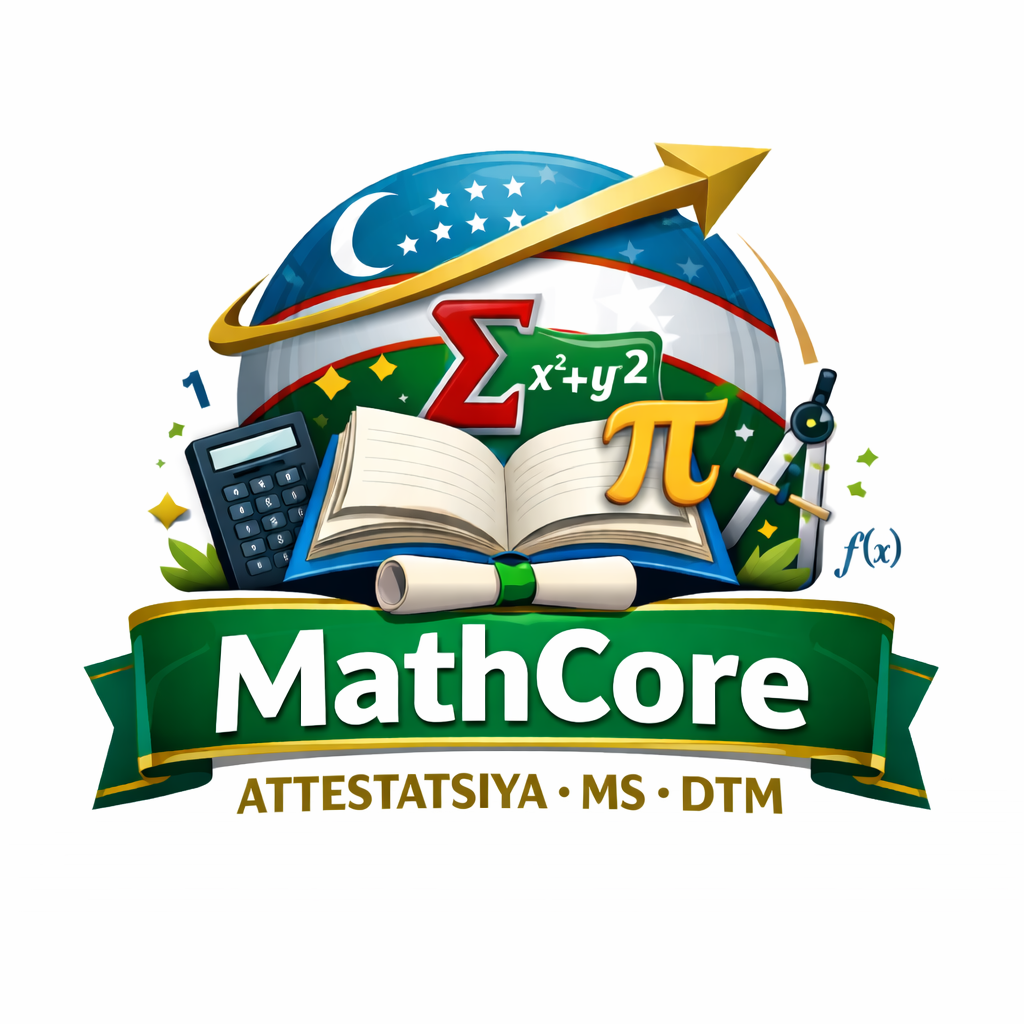
\includegraphics[width=0.3\textwidth]{logo.png}
\end{center}
\vspace{1cm}

% 1-masala
\begin{taskbox}
Nargiza 46 ta masala ishladi. Har bir to'g'ri javob uchun 5 ball beriladi va har bir noto'g'ri javob uchun 12 ball ayriladi. Agar u 77 ball to'plagan bo'lsa, nechta masalaga to'g'ri javob bergan?
\begin{tasks}(2)
\task 43
\task 41
\task 39
\task 37
\end{tasks}
\end{taskbox}

% 2-masala
\begin{taskbox}
Ikki ishchi birgalikda ishni 12 kunda tugatadi. Agar birinchi ishchi ishning yarmini bajarib, so'ngra ikkinchi ishchi qolgan yarmini bajarsa, ish 25 kunda tugaydi. Birinchi ishchi ikkinchisiga nisbatan necha marta tez ishlaydi?
\begin{tasks}(2)
\task 2
\task 1,5
\task 1,8
\task 2,5
\end{tasks}
\end{taskbox}

% 3-masala
\begin{taskbox}
To'g'ri prizmaning hajmi 40 ga teng. Unga hajmi $\frac{32\pi}{3}$ bo'lgan shar ichki chizilgan. Prizmaning yon sirti yuzini toping.
\begin{tasks}(2)
\task 10
\task 30
\task 40
\task 60
\end{tasks}
\end{taskbox}

% 4-masala
\begin{taskbox}
Birinchi va ikkinchi ishchi ishni 8 soatda, birinchi va uchinchi ishchi 12 soatda, ikkinchi va uchinchi ishchi 24 soatda tugatadi. Uchchalasi birgalikda necha soatda tugatadi?
\begin{tasks}(2)
\task 6
\task 16
\task 12
\task 8
\end{tasks}
\end{taskbox}

% 5-masala
\begin{taskbox}
$\tg 2x = \ctg 4x$ tenglamaning $[0; \pi]$ kesmadagi yechimlari soni nechta?
\begin{tasks}(2)
\task 3
\task 4
\task 5
\task 6
\end{tasks}
\end{taskbox}

% 6-masala
\begin{taskbox}
Tengsizlikni yeching: $|\lg x| < 1$.
\begin{tasks}(2)
\task $(10^{-1}; 10)$
\task $(0; 10)$
\task $(1; 10)$
\task $(10^{-2}; 10^{-1})$
\end{tasks}
\end{taskbox}

% 7-masala
\begin{taskbox}
$\lg x + \lg(x+6) = \lg(-a)$ tenglama $a$ ning qanday qiymatlarida yagona yechimga ega?
\begin{tasks}(2)
\task $\varnothing$
\task $a < 0$
\task $a \in \mathbb{R}$
\task $a \in (-7; 0)$
\end{tasks}
\end{taskbox}

% 8-masala
\begin{taskbox}
$\sin 4\pi x + \sin 2\pi x = 0$ tenglamaning $[0, 2\pi]$ kesmadagi butun yechimlari soni nechta?
\begin{tasks}(2)
\task 1
\task 3
\task 5
\task 7
\end{tasks}
\end{taskbox}

% 9-masala
\begin{taskbox}
$7^{201}$ ni 23 ga bo'lgandagi qoldiqni toping.
\begin{tasks}(2)
\task 1
\task 11
\task 17
\task 21
\end{tasks}
\end{taskbox}

% 9.5-masala (rasmli)
\begin{taskbox}
$\alpha$ burchakni toping.
\begin{center}
    \centering
    
\includegraphics[width=0.5\linewidth]{3.png}
\end{center}
\begin{tasks}(2)
\task $40^\circ$
\task $25^\circ$
\task $50^\circ$
\task $10^\circ$
\end{tasks}
\end{taskbox}

% 10-masala
\begin{taskbox}
Ko'paytuvchilarga ajrating: $(a+b+c)(ab+bc+ac) - abc$.
\begin{tasks}(2)
\task $(a+b)(b+c)(a+c)$
\task $(a+b+c)^2$
\task $(a+b+c)(a+b-c)$
\task $(a+b)(ab+bc+ac)$
\end{tasks}
\end{taskbox}

% 11-masala
\begin{taskbox}
$|7 - 6x - x^2| = 5a$ tenglama $a$ ning qanday qiymatlarida 3 ta yechimga ega?
\begin{tasks}(2)
\task $a \in (0; 3,2)$
\task $a = 3,2$
\task $a > 3,2$
\task $a = 0$
\end{tasks}
\end{taskbox}

% 12-masala
\begin{taskbox}
Agar $a, b, c$ turli raqamlar bo'lib, ular uchun $\overline{aabc} = (a+b+c)^3$ (bu yerda $\overline{aabc}$ to'rt xonali son) tenglik o'rinli bo'lsa, $a+b-c$ qiymatini toping.
\begin{tasks}(2)
\task 8
\task 6
\task 4
\task 5
\end{tasks}
\end{taskbox}

% 13-masala
\begin{taskbox}
Teng yonli uchburchakning asosiga tushirilgan balandligi 20 ga, asosi 30 ga teng. Yon tomoniga tushirilgan balandlikni toping.
\begin{tasks}(2)
\task 25
\task 24
\task 15
\task 18
\end{tasks}
\end{taskbox}

% 15-masala
\begin{taskbox}
Tenglamalar sistemasidan $xyz$ ni toping:
\[
\begin{cases}
x + y + z = 6\\
x - y + z = 4\\
z + y - x = 0
\end{cases}
\]
\begin{tasks}(2)
\task 2
\task 4
\task 6
\task 0
\end{tasks}
\end{taskbox}

% 16-masala
\begin{taskbox}
46 o'quvchi 10 ta qayiqqa chiqdi. Qayiqlar 6 o'rinli va 4 o'rinli bo'lsa, nechta o'quvchi 4 o'rinli qayiqlarda bo'lgan?
\begin{tasks}(2)
\task 7
\task 6
\task 24
\task 28
\end{tasks}
\end{taskbox}

% 17-masala
\begin{taskbox}
Ikki xonali sonlardan nechtasi 3 ga ham, 4 ga ham bo'linmaydi?
\begin{tasks}(2)
\task 50
\task 46
\task 40
\task 52
\end{tasks}
\end{taskbox}

% 18-masala
\begin{taskbox}
Natural sonlar qatori har bir natural sonning kvadrati bilan tugaydigan qismlarga ajratilgan: $\{1\}$, $\{2;3;4\}$, $\{5;6;7;8;9\}$, $\{10;11;12;13;14;15;16\}$, ... 10-guruhdagi sonlar yig'indisini toping.
\begin{tasks}(2)
\task 1626
\task 1729
\task 1758
\task 1800
\end{tasks}
\end{taskbox}

% 18.5-masala (rasmli)
\begin{taskbox}
Aylananing markazidan B nuqtagacha bo'lgan masofani toping.
\begin{center}
    \centering
    
\includegraphics[width=0.4\linewidth]{2.png}
\end{center}
\begin{tasks}(2)
\task 15
\task 14
\task 13
\task 12
\end{tasks}
\end{taskbox}

% 19-masala
\begin{taskbox}
$y = \lg(\cos x)$ funksiyaning qiymatlar sohasini toping.
\begin{tasks}(2)
\task $E(y) = (-\infty; 0]$
\task $E(y) = (-1; 0]$
\task $E(y) = (0; \infty)$
\task $E(y) = (-\infty; \infty)$
\end{tasks}
\end{taskbox}

% 20-masala
\begin{taskbox}
$\sin 4x + \cos 2x = 0$ tenglamani nechta o'tkir burchak ($x \in (0; \frac{\pi}{2})$) qanoatlantiradi?
\begin{tasks}(2)
\task 1
\task 2
\task 3
\task 4
\end{tasks}
\end{taskbox}

% 21-masala
\begin{taskbox}
Hisoblang: $\dfrac{3\lg 2 + 3\lg 5}{\lg 1300 - \lg 0,13}$.
\begin{tasks}(2)
\task $1,5$
\task $1,25$
\task $0,75$
\task $0,5$
\end{tasks}
\end{taskbox}

% 22-masala
\begin{taskbox}
$\tg 2x = \ctg 4x$ tenglamaning $[0; \pi]$ kesmadagi ildizlari yig'indisini toping.
\begin{tasks}(2)
\task $\dfrac{35\pi}{12}$
\task $\dfrac{11\pi}{4}$
\task $2\pi$
\task $\dfrac{13\pi}{6}$
\end{tasks}
\end{taskbox}

% 23-masala
\begin{taskbox}
$y = \lg(\arcsin x)$ funksiyaning qiymatlar sohasini toping.
\begin{tasks}(2)
\task $E(y) = (-\infty; \lg 2]$
\task $E(y) = (-\infty; 0]$
\task $E(y) = (0; \infty)$
\task $E(y) = (-\infty; \infty)$
\end{tasks}
\end{taskbox}

% 24-masala
\begin{taskbox}
Kesik konusning asos radiuslari 11 va 27 ga teng. Yasovchining balandlikka nisbati $17:15$ bo'lsa, uning o'q kesimi yuzini toping.
\begin{tasks}(2)
\task 760
\task 1140
\task 1260
\task 1440
\end{tasks}
\end{taskbox}

% 14-masala
\begin{taskbox}
Teng yonli uchburchakning yon tomoni 15 ga, asosiga tushirilgan balandligi 12 ga teng. Yon tomoniga tushirilgan balandlik uzunligini toping.
\begin{tasks}(2)
\task 14,4
\task 15
\task 16,2
\task 18
\end{tasks}
\end{taskbox}

% 25-masala
\begin{taskbox}
$y = |x-1| + |x-3|$ funksiyaning qiymatlar sohasini toping.
\begin{tasks}(2)
\task $E(y) = (2; \infty]$
\task $E(y) = (-\infty; 0]$
\task $E(y) = [2; \infty)$
\task $E(y) = (-\infty; \infty)$
\end{tasks}
\end{taskbox}

% 26-masala (takroriy raqam, 26.1)
\begin{taskbox}
To'g'ri prizma hajmi 40 ga, unga ichki chizilgan shar hajmi $\frac{32\pi}{3}$ ga teng. Prizmaning yon sirti yuzining shar sirti yuziga nisbatini toping.
\begin{tasks}(2)
\task $\dfrac{10}{5\pi}$
\task $\dfrac{10}{3\pi}$
\task $\dfrac{5}{2\pi}$
\task $\dfrac{5}{2\pi}$
\end{tasks}
\end{taskbox}

% 27-masala
\begin{taskbox}
$1 < |x-2| < 3$ tengsizlik nechta butun yechimga ega?
\begin{tasks}(2)
\task 0
\task 1
\task 2
\task 3
\end{tasks}
\end{taskbox}

% 26-masala (rasmli)
\begin{taskbox}
G nuqta ABC uchburchakning og'irlik markazi. Agar $AG \perp CG$, $CG=15$, $BG=20$ bo'lsa, BGC uchburchak yuzini toping.
\begin{center}
    \centering
    
\includegraphics[width=0.5\linewidth]{1.png}
\end{center}
\begin{tasks}(2)
\task $\dfrac{75\sqrt{7}}{2}$
\task $\dfrac{77\sqrt{7}}{2}$
\task $36\sqrt{5}$
\task $37\sqrt{5}$
\end{tasks}
\end{taskbox}

% 28-masala
\begin{taskbox}
$|x|(x^2 - 4) = -1$ tenglama nechta yechimga ega?
\begin{tasks}(2)
\task 1
\task 2
\task 3
\task 4
\end{tasks}
\end{taskbox}

% 28.5-masala (rasmli)
\begin{taskbox}
$ABC$ uchburchakda $BD$ - bissektrisa, $\angle BAC = 30^{\circ}$, $\angle BCA = 45^{\circ}$ va $DC = 8\sqrt{2}$ bo'lsa, $AD$ kesma uzunligini toping.
\begin{center}
    \centering
    
\includegraphics[width=0.5\linewidth]{4.png}
\end{center}
\begin{tasks}(2)
\task 12
\task 14
\task 16
\task \(16 \sqrt{2}\)
\end{tasks}
\end{taskbox}

% 29-masala
\begin{taskbox}
Asoslari parallel tekisliklarda yotuvchi va umumiy balandlikka ega bo'lgan ikkita konus berilgan. Asos radiuslari 4 va 6 ga teng. Agar $H = 15$ bo'lsa, konuslarning umumiy qismi hajmini toping.
\begin{tasks}(2)
\task $\dfrac{144\pi}{5}$
\task $40\pi$
\task $\dfrac{216\pi}{5}$
\task $60\pi$
\end{tasks}
\end{taskbox}

% 30-masala
\begin{taskbox}
Medianalari 9, 12 va 15 bo'lgan uchburchak yuzini toping.
\begin{tasks}(2)
\task 80
\task 72
\task 64
\task 60
\end{tasks}
\end{taskbox}

% 2-masala (takroriy, 2.1)
\begin{taskbox}
$ABC$ muntazam uchburchak berilgan. $AC$ tomonda $AK = KL = LC = 4$ bo'ladigan $K$ va $L$ nuqtalar olingan. Bo'yalgan soha yuzini toping.
\begin{center}
    \centering
    
\includegraphics[width=0.4\linewidth]{5.png}
\end{center}
\begin{tasks}(2)
\task \(12 \sqrt{3}\)
\task \(15 \sqrt{3}\)
\task \(18 \sqrt{3}\)
\task \(24 \sqrt{3}\)
\end{tasks}
\end{taskbox}

\end{document}